\documentclass{article}
\usepackage[T1]{fontenc}
\usepackage{lmodern}
\usepackage{amssymb,amsmath}
\usepackage{ifxetex,ifluatex}
\usepackage{fixltx2e} % provides \textsubscript
\usepackage{unicode-math}
\usepackage{booktabs}
\usepackage{minted}
\usepackage{float}
\usepackage{listings}
\usepackage[a4paper,left=3cm,right=2cm,top=2.5cm,bottom=2.5cm]{geometry}
% use upquote if available, for straight quotes in verbatim environments
\IfFileExists{upquote.sty}{\usepackage{upquote}}{}
\ifnum 0\ifxetex 1\fi\ifluatex 1\fi=0 % if pdftex
  \usepackage[utf8]{inputenc}
\else % if luatex or xelatex
  \ifxetex
    % \usepackage{mathspec} % conflicts with unicode-math
    \usepackage{xltxtra,xunicode}
  \else
    \usepackage{fontspec}
  \fi
  \defaultfontfeatures{Mapping=tex-text,Scale=MatchLowercase}
  \newcommand{\euro}{€}
    \setmonofont[Mapping=tex-ansi]{DejaVu Sans Mono}
\fi
% use microtype if available
\IfFileExists{microtype.sty}{\usepackage{microtype}}{}
\usepackage{graphicx}
% Redefine \includegraphics so that, unless explicit options are
% given, the image width will not exceed the width of the page.
% Images get their normal width if they fit onto the page, but
% are scaled down if they would overflow the margins.
\makeatletter
\def\ScaleIfNeeded{%
  \ifdim\Gin@nat@width>\linewidth
    \linewidth
  \else
    \Gin@nat@width
  \fi
}
\makeatother
\let\Oldincludegraphics\includegraphics
{%
 \catcode`\@=11\relax%
 \gdef\includegraphics{\@ifnextchar[{\Oldincludegraphics}{\Oldincludegraphics[width=\ScaleIfNeeded]}}%
}%
\ifxetex
  \usepackage[setpagesize=false, % page size defined by xetex
              unicode=false, % unicode breaks when used with xetex
              xetex]{hyperref}
\else
  \usepackage[unicode=true]{hyperref}
\fi
\hypersetup{breaklinks=true,
            bookmarks=true,
            pdfauthor={Oscar Felipe Toro, Adam Schønemann},
            pdftitle={Automatic Software Analysis - A General Framework},
            colorlinks=true,
            citecolor=blue,
            urlcolor=blue,
            linkcolor=magenta,
            pdfborder={0 0 0}}
\urlstyle{same}  % don't use monospace font for urls
\setlength{\parindent}{0pt}
\setlength{\parskip}{6pt plus 2pt minus 1pt}
\setlength{\emergencystretch}{3em}  % prevent overfull lines
\setcounter{secnumdepth}{5}

\title{Automatic Software Analysis - A General Framework}
\author{Oscar Felipe Toro, Adam Schønemann}
\date{}

\begin{document}
\maketitle

\section{Introduction}\label{introduction}

This report will elaborate on the design and implementation of a general
framework for defining automatic software analyses on a small
toy programming language (C--). The framework is implemented in Haskell.

\section{Overview}\label{overview}

Software analysis is the process of taking a program as input, analysing
that program and then giving an approximation of a property of that program.
This approximation can in turn be used to optimize the program, guide
the programmer, or warn the programmer about potential errors.

\section{Modeling the Language}\label{modeling-the-language}

In order to to analyze a program, one needs a concrete representation of
that program as data, i.e. the Abstract Syntax Tree (AST).
The programming language we'll be analysing in this report, is
the simple language called C--. The syntax for C-- is defined by the
following grammar (Figure \ref{cmm-grammar}):
\begin{figure}[H]
\centering
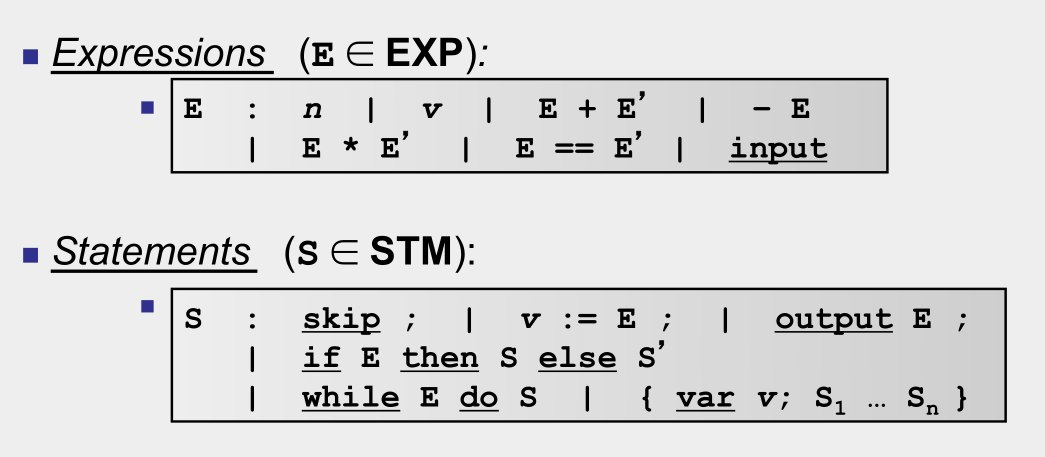
\includegraphics{./imgs/cmm.jpg}
\caption{Grammar for C--}
\label{cmm-grammar}
\end{figure}

In Haskell, we can use Algebraic Datatypes to model this grammar (Listing \ref{cmm-ast}):

\begin{listing}[H]
\begin{minted}{haskell}
-- Expression grammar
data Expr
  = Add Expr Expr
  | Sub Expr Expr
  | Mul Expr Expr
  | Gt  Expr Expr
  | Lt  Expr Expr
  | Eq  Expr Expr
  | BLit Bool
  | ILit Int
  | Var String
  | Input

-- Grammar for "simple" statements
data Stmt
  = Skip
  | Ass String Expr
  | Output Expr

-- Grammar for compound statements (or sub-programs)
data SubProg
  = ITE Expr SubProg SubProg
  | Block [SubProg]
  | While Expr SubProg
  | Single Stmt

type Program = [SubProg]
\end{minted}
\caption{C-- AST data types}
\label{cmm-ast}
\end{listing}

Note some discrepancies between the grammar and the Haskell data-types:

\begin{itemize}
\itemsep1pt\parskip0pt\parsep0pt
\item
  The expression grammar contains some extra operators as well as the
  Boolean literals
\item
  The grammar for statements has been split in two:

  \begin{itemize}
  \itemsep1pt\parskip0pt\parsep0pt
  \item
    Simple statements (\texttt{Output}, \texttt{Assign} and
    \texttt{Skip})
  \item
    Compund statements (\texttt{ITE}, \texttt{While}, \texttt{Block})

    \begin{itemize}
    \itemsep1pt\parskip0pt\parsep0pt
    \item
      These are statements that contain other statements. They can be
      considered ``sub-programs''
    \end{itemize}
  \end{itemize}
\item
  The variable declaration syntax (\texttt{var v;}) has been omitted,
  for simplicity
\end{itemize}

The reason for splitting the Statement grammar in two, is to have better
type-safety guarantees when implementing some algorithms later.
Semantically, it is also beneficial to distinguish between simple and
compound statements.

\subsubsection{Parsing}\label{parsing}

In order to work with programs in C--, the programmer will write
programs in textual form, and a parser will take care of converting this
form to the Haskell representation shown above. An excerpt of the parser
is shown below (Listing \ref{parser}).

\begin{listing}[H]
\begin{minted}{haskell}
program :: Parser Program
program = spaces *> many (stmt <* spaces)

stmt :: Parser SubProg
stmt =  (const $ Single Skip) <$> trystring "skip" <* spaces <* char ';' <* spaces
    <|> ITE <$> (trystring "if" *> spaces1 *> expr) <*>
                     (trystring "then" *> spaces1 *> stmt <* spaces) <*>
                     (trystring "else" *> spaces1 *> stmt <* spaces)
    <|> While <$> (trystring "while" *> spaces1 *> expr) <*>
                     (trystring "do" *> spaces1 *> stmt) <* spaces
    <|> (Single . Output) <$>
            (trystring "output" *> spaces1 *> expr <* char ';') <* spaces
    <|> (\v e -> Single $ Ass v e) <$>
            ident <* spaces) <*>
            (string ":=" *> spaces *> expr <* char ';') <* spaces
    <|> Block <$> (brackets block) <* spaces
      where
        block = sepBy stmt spaces
\end{minted}
\caption{The C-- parser}
\label{parser}
\end{listing}

The parser is implemented using the \texttt{Parsec} library. Since we do
not use a lexer, we have to be careful with the spaces - but otherwise,
the parser very closely resembles the grammar. Below is an example
program in C-- and its corresponding AST (Listing \ref{ast}).

\begin{listing}[H]
\begin{minted}{haskell}
x := 0;
y := 2;
while x < 10 do {
  x := x + 1;
  y := y * y;
}
output y;

-- AST
[ Single (Ass "x" (ILit 0))
, Single (Ass "y" (ILit 2))
, While (Lt (Var "x") (ILit 10))
     (Block [ Single (Ass "x" (Add (Var "x") (ILit 1)))
            , Single (Ass "y" (Mul (Var "y") (Var "y")))
            ])
, Single (Output (Var "y"))
]
\end{minted}
\caption{Program and corresponding AST}
\label{ast}
\end{listing}

\section{Control-Flow Graph}\label{control-flow-graph}

Once we have a concrete model of a program, we can perform analyses on
this model. To do so, we can create a control-flow graph (CFG) of the
program, that represents the order in which the statements in the program is
executed. Below is the control-flow graph corresponding to the program
above (Figure \ref{cfg-fig}).

\begin{figure}[H]
\centering
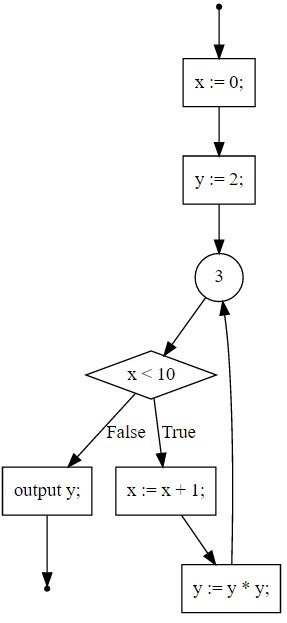
\includegraphics{./imgs/in10-cfg.jpg}
\caption{Control-Flow graph of the program in Listing \ref{ast}}
\label{cfg-fig}
\end{figure}

In Haskell, the control-flow graph is modeled as a \texttt{Map} from
\texttt{ID} (an \texttt{Int}) to a \texttt{Node} (Listing \ref{cfg-hask}).

\begin{listing}[H]
\begin{minted}{haskell}
type ID = Int
type In = ID
type Out = ID
type BrTrue = ID
type BrFalse = ID
type End = ID

data Node
  = NSource Out
  | NSingle Stmt In Out
  | NITE Expr In BrTrue BrFalse End -- end of the conditional (points to confluence)
  | NWhile Expr In BrTrue BrFalse End -- end of the conditional (points to confluence)
  | NConfl (In, In) Out
  | NSink In
\end{minted}
\caption{CFG data types}
\label{cfg-hask}
\end{listing}

As can be seen in the code, a \texttt{Node} in the graph is either a
\texttt{NSource} (the start of the program), a \texttt{NSingle} (a node
containing a single statement), a \texttt{NITE} representing an
if-then-else statement, a \texttt{NWhile} (a while statement), a
\texttt{NConfl}, which is a confluence node, or, finally, a
\texttt{NSink} which is the end of the program.

Notice that the nodes themselves contain their in- and out-going edges.
This representation, rather than a more general graph-representation,
with a set of nodes and edges, allows for better performance and more
type-safety, as the types guarantee the number of edges going in-and-out
of the nodes, which statically prevents the construction of most
non-wellformed graphs.

Along with the data types are functions that can transform the
AST of a C-- program to its corresponding CFG
(\texttt{Program -\textgreater{} CFG}) and the inverse function
(\texttt{CFG -\textgreater{} Program})

\section{The Analysis}\label{the-analysis}

Given the CFG of a program you can perform a number of different
analyses on that program. In order to define analyses in a declarative
and concise manner, we have attempted to create an analysis framework that
is independent of the specific analyses. To do this, we have defined
some typeclasses and data types that allows users of the framework to
define their own analyses declaratively.

\subsection{The Lattice}\label{the-lattice}

Central to any analysis is the type of lattice that is used. Formally, a
lattice is a \textbf{partial order} with an operation $⊔S$ (called
\emph{join} or \emph{least upper bound}) that exists for all subsets
$S ⊆ L$. For finite lattices (which we are interested in, only), $⊔$
need only be defined for each \textbf{pair} of elements in $S$.

A partial order is defined as a structure $(S, ⊑)$ where $S$ is a set
and $⊑$ is a binary relation on $S$ that satisfies:

\begin{itemize}
\itemsep1pt\parskip0pt\parsep0pt
\item
  Reflexivity: $∀x ∈ S.\; x ⊑ x$
\item
  Transitivity: $∀x,y,z ∈ S.\;  x ⊑ y ∧ y ⊑ z ⇒ x ⊑ z$
\item
  Anti-Symmetry: $∀x,y ∈ S.\; x ⊑ y ∧ y ⊑ x ⇒ x = y$
\end{itemize}

To generalise this concept, we have defined a lattice typeclass called
\texttt{Lat} (Listing \ref{lat-lst}).

\begin{listing}[H]
\begin{minted}{haskell}
class (Ord a, Eq a, Show a) => Lat a where
  bottom          :: Program -> a
  leastUpperBound :: a -> a -> a
  top             :: Program -> a

-- the simplest lattice possible (one-element lattice)
data UnitLat = UnitLat deriving (Ord, Eq, Show)

instance Lat UnitLat where
  bottom              = const UnitLat
  leastUpperBound _ _ = UnitLat
  top                 = const UnitLat
\end{minted}
\caption{The Lattice typeclass}
\label{lat-lst}
\end{listing}

To make a data type an instance of the \texttt{Lat} typeclass, the
programmer will have to define the \texttt{top}, \texttt{bottom} and
\texttt{leastUpperBound} functions. The \texttt{top} and \texttt{bottom}
functions take a program as input, in order to dynamically generate the
top and bottom elements specific to that program. The constraints
\texttt{Ord a} and \texttt{Eq a} on the typeclass definition make sure
that a partial order is defined for the type parameter \texttt{a} before
you can instance it as a lattice.

\subsection{The Analysis Type}\label{the-analysis-type}

An analysis is represented as a concrete record, whose arguments are
1) a mapping from a CFG $\mathtt{Node}$ to a corresponding transfer function, and 2) a function that resolves dependencies of program-points in the graph
(Listing \ref{anal}).

\begin{listing}[H]
\begin{minted}{haskell}
data Analysis a
  = Analysis { nodeToTFun :: Node -> TFun a
             , getDeps    :: Node -> Map ID a -> a
             }
\end{minted}
\caption{The Analysis record}
\label{anal}
\end{listing}

\texttt{getDeps} can be used to specify if the analysis is a backwards-
or forwards-analysis, but in practice it allows for even more complex
data flows, if the need should arise. Listing \ref{back-forwd} presents the
backwards and forward combinators.

\begin{listing}[H]
\begin{minted}{haskell}
-- combinator for forward analyses
forward :: Lat a => a -> Node -> Map ID a -> a
forward srcEnv node envs =
  case node of
      NSource o          -> srcEnv
      NSingle stmt i o   -> getEnv i
      NITE e i bt bf _   -> getEnv i
      NWhile e i bt bf _ -> getEnv i
      NConfl (i1, i2) o  -> leastUpperBound (getEnv i1) (getEnv i2)
      NSink i            -> getEnv i
  where getEnv k = unsafeLookup k envs

-- combinator for backwards analyses
backwards :: Lat a => a -> Node -> Map ID a -> a
backwards sinkEnv node envs =
  case node of
      NSource o          -> getEnv o
      NSingle stmt i o   -> getEnv o
      NITE e i bt bf _   -> leastUpperBound (getEnv bt) (getEnv bf)
      NWhile e i bt bf _ -> leastUpperBound (getEnv bt) (getEnv bf)
      NConfl (i1, i2) o  -> getEnv o
      NSink i            -> sinkEnv
  where getEnv k = unsafeLookup k envs
\end{minted}
\caption{The backwards and forwards combinator}
\label{back-forwd}
\end{listing}

As an example, the complete implementation of the ``Live Variable'', or
``Liveness'' analyses can be seen below (Figure \ref{liveness}):

\begin{listing}[H]
\begin{minted}{haskell}
newtype LiveEnv = LEnv { unLive :: (Set String) } deriving (Ord, Eq, Show)

instance Lat LiveEnv where
  leastUpperBound a b = LEnv $ S.union (unLive a) (unLive b)
  bottom              = const (LEnv S.empty)
  top                 = LEnv . collectVars

liveNodeToTFun :: Node -> TFun LiveEnv
liveNodeToTFun node = case node of
    NSingle stmt _ _ ->
      case stmt of
        Skip     -> id
        Ass v e  -> union (vars e) . delete v
        Output e -> union (vars e)
    NITE   e _ _ _ _ -> exprToTFun e
    NWhile e _ _ _ _ -> exprToTFun e
    node'            -> id
  where
    exprToTFun e = LEnv . S.union (unLive . vars $ e) . unLive
    union e      = LEnv . S.union (unLive e) . unLive
    delete v     = LEnv . S.delete v . unLive

vars :: Expr -> LiveEnv
vars = LEnv . help where
  help expr =
    case expr of
      Add e1 e2 -> help e1 `S.union` help e2
      Sub e1 e2 -> help e1 `S.union` help e2
      Mul e1 e2 -> help e1 `S.union` help e2
      Gt  e1 e2 -> help e1 `S.union` help e2
      Lt  e1 e2 -> help e1 `S.union` help e2
      Eq  e1 e2 -> help e1 `S.union` help e2
      BLit b    -> S.empty
      ILit i    -> S.empty
      Var n     -> S.singleton n
      Input     -> S.empty

livenessAnal :: Analysis LiveEnv
livenessAnal =
  Analysis { nodeToTFun = liveNodeToTFun
           , getDeps    = backwards (LEnv S.empty)
           }
\end{minted}
\caption{The complete implementation for the Live Variables analysis}
\label{liveness}
\end{listing}

\subsection{Program-Points}\label{program-points}

After constructing the CFG of a program, one would generate
program-points from this CFG. The program-points represent the result of
the analysis at a specific point of the execution of the program. A
program-point has an associated transfer-function that -- given an
``environment lattice'' that represents the result of the analysis at a
previous program-point -- updates the result to reflect the effect of the
statement at the current program-point.

In our implementation, we have chosen not to model program-points as an
explicit data type, but implicitly in terms of the recursive equations
derived from the control-flow graph.

\subsection{Recursive Equations}\label{recursive-equations}

From each program point and its associated transfer function, an
equation that encodes how the analyses progresses from each
program-point (or statement) to the next should be generated.

\begin{minted}{haskell}
-- a function from dependencies to a single lattice element
type Equation a = Map ID a -> a
\end{minted}

An equation over the type parameter \texttt{a} is simply modeled as a
function from a \texttt{Map ID a} to \texttt{a}. That is, the equation
receives a map from program-point IDs to their corresponding lattice
elements, and produces a new lattice element according to its
dependencies. For example, in the CFG above, the equation corresponding
to the statement \texttt{y := 2;} would take a \texttt{Map} containing
the results of the previous iteration of the fixed-point algorithm,
select the lattice element corresponding to \texttt{x := 0;} and apply
its associated transfer function to that lattice element. In case of
e.g.~the ``Available Expressions'' analysis, given that the ID of
\texttt{x := 0;} is $1$ the equation for \texttt{y := 2;} would be
\texttt{\textbackslash{}env -\textgreater{} assign "y" (ILit 2) (lookup 1 env)}.

Consequently, given that the example program we've used so far (Listing \ref{ast}) yields
the following recursive equations: \begin{equation}
\begin{array}{lll}
⟦entry⟧   &=& \emptyset \\
⟦x := 0;⟧ &=& ⟦entry⟧ ∪ assign_x(0) \\
⟦y := 2;⟧ &=& ⟦x := 0;⟧ ∪ assign_y(2) \\
⟦x < 10⟧  &=& (⟦y := 2;⟧ ∩ ⟦y := y * y;⟧) ∪ exprs(x < 10) \\
⟦x := x + 1;⟧ &=& ⟦x < 10⟧ ∪ assign_x(x + 1) \\
⟦y := y * y;⟧ &=& ⟦x := x + 1;⟧ ∪ assign_y(y * y) \\
⟦\mathtt{output\ }y;⟧   &=& ⟦x < 10⟧ ∪ exprs(y)
\end{array}
\end{equation}

the Haskell representation can be conceptualized as follows (Listing \ref{rec-eq}):

\begin{listing}[H]
\begin{minted}{haskell}
case nodeId of
    0 -> \env -> S.empty                                                -- entry
    1 -> \env -> (get 0 env) `union` assign "x" (ILit 0)                -- x := 0;
    2 -> \env -> (get 1 env) `union` assign "y" (ILit 2)                -- y := 2;
    3 -> \env -> leastUpperBound (get 2 env) (get 6 env)                -- confluence
    4 -> \env -> (get 3 env) `union` exprs (Var "x" `Lt` (ILit 10))     -- x < 10
    5 -> \env -> (get 4 env) `union` assign "x" (Var "x" `Add` Lit 1)   -- x := x + 1
    6 -> \env -> (get 5 env) `union` assign "y" (Var "y" `Mul` Var "y") -- y := y * y
    7 -> \env -> (get 4 env) `union` exprs (Var "y")                    -- output y
    8 -> \env -> env                                                    -- sink
\end{minted}
\caption{Conceptual Haskell code representing recursive equations}
\label{rec-eq}
\end{listing}

\subsection{Solving the equations using the fixed-point
theorem}\label{solving-the-equations-using-the-fixed-point-theorem}

Now that the equations have been modeled, we can easily build the ``big
transfer function''

\begin{minted}{haskell}
type BigT a = Map ID a -> Map ID a

eqsToBigT :: Lat a => Map ID (Equation a) -> BigT a
eqsToBigT eqs l = M.map ($ l) eqs
\end{minted}

and now, we can use this structure to solve the recursive equations
using the fixed-point theorem, translated to Haskell using the
\texttt{fix} combinator (Listing \ref{fixp-listing}).

\begin{listing}[H]
\begin{minted}{haskell}
-- fixpoint operator!
fix :: (a -> a) -> a
fix f =
  let x = f x
  in  x

-- solveFix without explicit recursion
solveFix :: Lat a => Map ID a -> BigT a -> Map ID a
solveFix = fix (\f l bigT ->
                   let l' = bigT l
                   in if (l == l') then l else f l' bigT
                )
\end{minted}
\caption{Solve equations using the fixed-point theorem}
\label{fixp-listing}
\end{listing}

Here, Haskell's lazy evaluation allows us to translate the mathematical
definition of the fixpoint combinator almost verbatim.

To run an analysis on a program, a user of the framework can call the
\texttt{analyzeProg} function

\begin{minted}{haskell}
-- takes an analysis over a lattice element, and a program.
-- returns a Map from CFG Node ID to least solution to the analysis
analyzeProg :: Lat a => Analysis a -> Program -> Map ID a
analyzeProg anal prog = solveFix initial bigT where
  cfg@(CFG nodes) = progToCfg prog
  initialL = bottom prog
  eqs = cfgToEqs anal cfg
  bigT = eqsToBigT eqs
  initial = M.map (const initialL) nodes
\end{minted}

\subsection{Lattice typeclass and
ordering}\label{lattice-typeclass-and-ordering}

The observant reader will notice that the partial order required in the
lattice typeclass is not actually used anywhere. In theory, this order is
necessary to prove monotonicity of the transfer functions used in an
analysis. In principle, we should require that, when defining a new
analysis, the user of the framework should also prove monotonicity of the
transfer functions, in order to guarantee that the fixed-point solver
terminates. This, however, is not possible within the type system of
Haskell. In order to do such a thing, one would require a language that
can encode logic in some form, through e.g.~dependent types.

\section{Implementing examples of
analyses}\label{implementing-examples-of-analyses}

In order to guide the design of our framework and test it, we've
implemented several different analyses, using different lattices,
operations and control-flow directions. This section will briefly
describe them.

\subsection{Available Expressions}\label{available-expressions}

\emph{Available Expressions} analyses a program in order to
re-use expressions that have already been evaluated. The lattice is a
set of expressions, and the least upper bound operation is simply set
intersection (Listing \ref{avail}).

\begin{listing}[H]
\begin{minted}{haskell}
instance Lat (Set Expr) where
  bottom          = collectExprs
  leastUpperBound = S.intersection
  top             = const S.empty

available :: Analysis (Set Expr)
available =
  Analysis { nodeToTFun = availNodeToTFun
           , getDeps = forward S.empty
           }
\end{minted}
\caption{The Lattice typeclass}
\label{avail}
\end{listing}

Notice here, in relation to the discussion about ordering of lattice
elements in section \ref{lattice-typeclass-and-ordering}, that the built-in \texttt{Ord} instance for \texttt{Set} is
ordered with $⊆$ and not $⊇$, which is the order specified for the
\emph{Available Expressions} analysis. However, in practice, as long as
our transfer functions actually are monotonous with respect to the
partial order defined by $⊇$, this is not an issue, and the fixed-point solve
will run and terminate happily.

\subsection{Live Variables}\label{live-variables}

\emph{Live Variables} analyses a program in order to
determine if, and when, variables are used. If they are not used, we can omit
writes to the variables that are never seen. Since we have already show
the full code for \emph{Live Variables} previously in this
report (Listing \ref{liveness}), we will omit it at this point.

\subsection{Constant Propagation}

\emph{Constant Propagation} analyses a program in order to
determine which variables are actually constants, and what their constant
value is. This analysis can be used to defer some calculations to
compile-time. Additionally, it can be used to reveal branches of the
code that are never executed. The code excerpt below shows some of the definitions involved in implementing the analysis (Listing \ref{cp-listing}).

\begin{listing}[H]
\begin{minted}{haskell}
-- constant propagation lattice for a single variable
data CPLat
  = CPTop       -- we can't know if it is constant
  | CPBot       -- we don't know yet
  | CPInt  Int  -- it is a constant int
  | CPBool Bool -- it is a constant bool
  deriving (Show, Eq, Ord)

instance Lat CPLat where
  bottom = const CPBot
  leastUpperBound = cpLUP
  top    = const CPTop

-- map from variables to their CPLat values
type Env = Map String CPLat

instance Lat Env where
  bottom = M.fromList . S.toList . S.map (\v -> (v, CPBot)) . collectVars
  leastUpperBound = envLUP
  top = const M.empty

cpNodeToTFun :: Node -> TFun Env
cpNodeToTFun node = case node of
  NSingle stmt _ _  -> cpSingleToTFun stmt
  node'             -> id
where
  cpSingleToTFun stmt = case stmt of
    Skip     -> id
    Ass v e  -> \env -> M.insert v (evalExpr e env) env
    Output _ -> id

constProp :: Analysis Env
constProp =
  Analysis { nodeToTFun = cpNodeToTFun
           , getDeps = forward (M.empty)
           }
\end{minted}
\caption{Constant Propagation implementation}
\label{cp-listing}
\end{listing}

\section{Optimisations}\label{optimizations}

What good is an analysis, if we cannot use it for anything? Our
framework also contains functions and types that can be used to
implement optimisations directly on the AST of the program. These
optimisations are usually coupled to an analysis, and uses the result of
the analysis to transform the program into a different (hopefully
better) form.

An optimisation is represented by a record containing an analysis and a
way to transform the AST using that analysis

\begin{minted}{haskell}
data Optimization = forall a. Lat a =>
  Opt { optTransform  :: [Annotated a] -> Program
      , optAnalysis   :: Analysis  a
      }
\end{minted}

The \texttt{forall a.} syntax introduces an existential type - this
means we can use the type variable \texttt{a} on the right-hand side
without mentioning it in the type signature for \texttt{Optimization}.
This will later allow us to put optimisations using different analyses
in the same collection, so that we can chain multiple optimisations after
another.

The core data type that the transformations work on is the
\texttt{Annotated} type. \texttt{Annotated a} represents an AST that is
annotated with the result of an analysis \texttt{a} (Listing \ref{annotated}).

\begin{listing}[H]
\begin{minted}{haskell}
data Annotated a = ASingle a Stmt
                 | AITE a Expr (Annotated a) (Annotated a)
                 | AWhile a Expr (Annotated a)
                 | ABlock [Annotated a]

-- annotated algebra for folding
-- a is the annotated's type param
-- b is the type of the accumulator
data AnnAlg a b = AnnAlg
  { aaSubProg  :: a -> Stmt -> b -> b
  , aaITE      :: a -> Expr -> b -> b -> b -> b
  , aaWhile    :: a -> Expr -> b -> b -> b
  , aaBlock    :: [b] -> b -> b
  }

-- fold over an annotated using an AnnAlg
foldAnn         :: AnnAlg a b -> b -> Annotated a -> b

-- intepret an Annotated into a new program
interpAnn       :: (a -> SubProg -> SubProg) -> Annotated a -> SubProg

-- strip the annotations
annotatedToProg :: [Annotated a] -> Program

-- convert a cfg along with the result of an analysis into a list of
-- annotated sub-programs
cfgToAnnotated  :: Lat a => Map ID a -> CFG -> [Annotated a]
\end{minted}
\caption{The Annotated data type}
\label{annotated}
\end{listing}

To run a single pass of an optimization on a program, a user can call
the \texttt{runOpt} function (Listing \ref{runopt}).

\begin{listing}[H]
\begin{minted}{haskell}
runOpt :: Optimization -> Program -> Program
runOpt (Opt trans anal) prog =
  let cfg       = progToCfg prog
      analyzed  = analyzeProg anal prog
      annotated = cfgToAnnotated analyzed cfg
      optimized = trans annotated
  in optimized

-- run optb first and then opt a
runOpts :: Optimization -> Optimization -> Program -> Program

-- run a list of optimizations in sequence (right to left)
seqOpts :: [Optimization] -> (Program -> Program)

-- use the fixed-point theorem again to optimize a program to its "most-optimized"
-- form
optimizeProg :: [Optimization] -> Program -> Program
optimizeProg opts prog =
  let fixpoint =
        fix (\f prog -> let prog' = seqOpts opts prog
                        in  if prog' == prog then prog' else f prog'
        )
  in  fixpoint prog
\end{minted}
\caption{Running an optimisation}
\label{runopt}
\end{listing}

\section{Dead-Code Elimination and Constant
Propagation}\label{dead-code-elimination-and-constant-propagation}

\emph{Dead-Code Elimination} is a powerful optimisation that allows for
eliminating entire branches of a program if we can deduce that it will
never be run. Dead-Code Elimination can significantly improve the
effectiveness of many other optimisations by removing large parts of the
program and thus simplifying the control-flow substantially.

Dead-Code elimination by itself is not particularly smart - it will only
eliminate branches whose conditional is constantly true or false.
However, in combination with \emph{Constant Propagation}, its
effectivity is significantly improved, since Constant Propagation will
reveal any expressions that are constant, and reduce them to their
constant values.

\subsection{Constant Propagation}\label{constant-propagation-1}

Below is an excerpt of the implementation of the Constant Propagation
optimisation (Listing \ref{cp-opt-impl}).

\begin{listing}[H]
\begin{minted}{haskell}
-- a transformation from annotated AST to a AST with all constant expressions
-- replaced with their constants
cpTransform :: [Annotated Env] -> Program
cpTransform anns = map (interpAnn stmt) anns where
  stmt :: Env -> SubProg -> SubProg
  stmt env st = case st of
    Single (Skip    ) -> Single Skip
    Single (Ass v e ) -> Single $ Ass v (expr env e)
    Single (Output e) -> Single $ Output (expr env e)
    ITE e bt bf       -> ITE (expr env e) bt bf
    Block ss          -> Block ss
    While e s         -> While (expr env e) s
  expr :: Env -> Expr -> Expr
  expr env e = maybe e id (cLatToMaybeExpr . isConst env $ e) where
    ...

constPropOpt :: Optimization
constPropOpt =
  Opt { optTransform  = cpTransform
      , optAnalysis   = constProp
      }
\end{minted}
\caption{Implementation of the Constant Propagation optimisation}
\label{cp-opt-impl}
\end{listing}
The transformation will iterate through the annotated source, and when
it encounters an expression it will attempt to replace it with its
constant literal. It uses the result of the Constant Propagation analysis in
order to do this.

\subsection{Dead-Code Elimination}\label{dead-code-elimination}

Below is the full implementation of the Dead-Code elimination
optimisation (Listing \ref{dead-code}).

\begin{listing}[H]
\begin{minted}{haskell}
deadCodeTransAnn :: [Annotated a] -> Program
deadCodeTransAnn = deadCodeTrans . annotatedToProg

-- we do not dependent on any analysis at all, so the transformation is
-- effectively from Program to Program (an endo-function!)
deadCodeTrans :: Program -> Program
deadCodeTrans ss = foldr dct [] ss where
  dct stmt acc =
    case stmt of
      Single _ -> stmt : acc
      ITE e bt bf ->
        case e of
          BLit True  -> dct bt acc
          BLit False -> dct bf acc
          _          -> ITE e (s2s $ dct bt []) (s2s $ dct bf []) : acc
      Block ss'   -> deadCodeTrans ss' ++ acc
      While e s   ->
        case e of
          BLit True  -> While e s : acc
          BLit False -> acc
          _          -> While e (s2s $ dct s []) : acc
  s2s = stmtsToSubProg

deadCodeOpt :: Optimization
deadCodeOpt =
  Opt { optTransform  = deadCodeTransAnn :: [Annotated UnitLat] -> Program
      , optAnalysis   = idAnalysis UnitLat
      }
\end{minted}
\caption{Dead-Code Elimination}
\label{dead-code}
\end{listing}

Note that the Dead-Code Elimination does not depend on any analysis.
Therefore, its corresponding analysis is just the \texttt{idAnalysis} -
the analysis that does nothing.

\subsection{Optimizations in Action}\label{optimizations-in-action}

Consider the C-- program below (Listing \ref{cmm-p1}):

\begin{listing}[H]
\begin{minted}{haskell}
x := 2 < 10;
if x then
  if false then
    y := true;
  else {
    y := false;
    z := 42 * 42;
  }
else
  y := 100 - (10 * 10);|]
\end{minted}
\caption{C-- program 1}
\label{cmm-p1}
\end{listing}

Running simply Dead-Code elimination will eliminate the inner if, and
produce the code below (Listing \ref{cmm-p2}):

\begin{listing}[H]
\begin{minted}{haskell}
x := 2 < 10;
if x then
    y := false;
    z := 42 * 42;
else
  y := 100 - (10 * 10);|]
\end{minted}
\ref{cmm-p2}
\label{C-- program 2}
\end{listing}

However, running Constant Propagation first will reveal that \texttt{x}
is in fact constantly \texttt{true}, and thus the outer branch can also
be eliminated, resulting in (Listing \ref{cmm-p3}).

\begin{listing}[H]
\begin{minted}{haskell}
x := true;
y := false;
z := 1764;
\end{minted}
\caption{C-- program 3}
\label{cmm-p3}
\end{listing}

The resulting program is drastically simplified.

Running the two optimizations inside a fixpoint can even eliminate dead
code in quite sophisticated cases, such as in Listing \ref{cmm-p4}.

\begin{listing}[H]
\begin{minted}{haskell}
a := (20 * 3) - 1;
b := a + 9;
c := 0;
while b < 68 do {
  output a * b;
  if (10 + a) > 41 then
    output c;
  else {
    c := c + 1;
    b := a;
  }
}
output c + a;
\end{minted}
\caption{C-- program 4}
\label{cmm-p4}
\end{listing}

Simply running Constant Propagation once will yield Listing \ref{cmm-p5}:

\begin{listing}[H]
\begin{minted}{haskell}
a := 59;
b := 68;
c := 0;
while b < 68 do {
  output a * b;
  if true then
    output c;
  else {
    c := c + 1;
    b := 59;
  }
}
output c + a;
\end{minted}
\caption{C-- program 5}
\label{cmm-p5}
\end{listing}

which does not reveal that \texttt{b} is in fact constant, because the
else branch of the inner if will never be executed. However, should we
run Dead-Code Elimination now, this fact will be revealed (Listing \ref{cmm-p6}):

\begin{listing}[H]
\begin{minted}{haskell}
a := 59;
b := 68;
c := 0;
while b < 68 do {
  output a * b;
  output c;
}
output c + a;
\end{minted}
\caption{C-- program 6}
\label{cmm-p6}
\end{listing}

Running Constant Propagation once more, we can now see that the
condition in the while loop is constantly false, and running Dead-Code
Elimination one more time produces the final code (Listing \ref{cmm-p7}):

\begin{listing}[H]
\begin{minted}{haskell}
a := 59;
b := 68;
c := 0;
output 59;
\end{minted}
\caption{C-- program 7}
\label{cmm-p7}
\end{listing}

\section{Future work}\label{future-work}

There are many things that could be improved in this framework. Some of
them are:

\begin{itemize}
\itemsep1pt\parskip0pt\parsep0pt
\item
  Analyze a more sophisticated language
\item
  Implement more analyses and optimizations
\item
  Consider requiring proofs of monotonicity
\item
  Optimize the fixed-point solver using e.g.~chaotic iteration
\end{itemize}

\end{document}
